\documentclass[border=5mm]{standalone}
\usepackage{tikz}
\usetikzlibrary{intersections}
\begin{document}
% We're working on
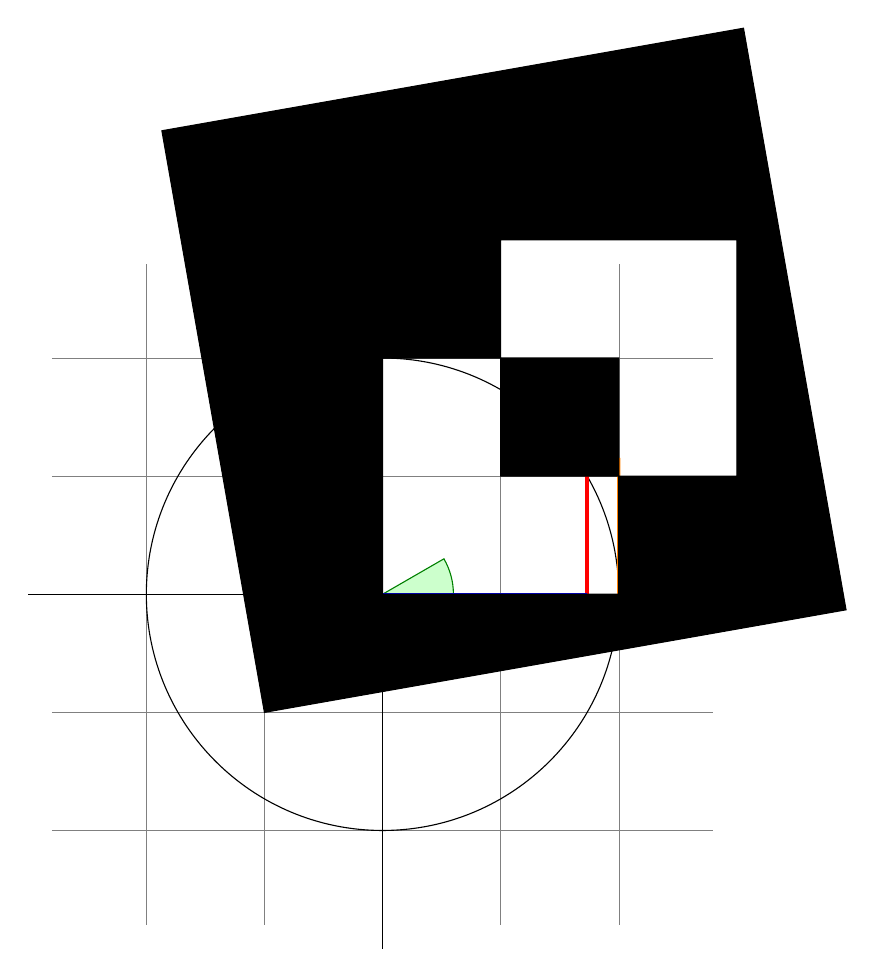
\begin{tikzpicture} [
  scale = 3,
]
\draw [
  step = .5,
  gray,
  very thin,
] (-1.4, -1.4) grid (1.4, 1.4);
\draw (-1.5, 0) -- (1.5, 0);
\draw (0, -1.5) -- (0, 1.5);
\draw (0, 0) circle [radius = 1];
\filldraw [fill = green!20!white, draw = green!50!black] (0, 0) -- (.3, 0) arc [start angle = 0, end angle = 30, radius = .3] -- cycle;
\draw [red, very thick] (30:1) -- (30:1 |- 0,0);
\draw [blue, very thick] (0, 0) -- (0,0 -| 30:1);

% Drawing the tan as an intersection
\path [name path = vert] (1, 0) -- (1, 1);
\path [name path = 30deg] (0, 0) -- (30:1.5);
\draw [name intersections = {of = vert and 30deg, by = t}, very thick, orange] (t) -- (1, 0);
\filldraw [even odd rule] (0,0) rectangle (1,1)
[xshift=5mm,yshift=5mm] (0,0) rectangle (1,1)
[xshift=-1cm,yshift=-1cm,scale=2.5,rotate=10] (0,0) rectangle (1,1);
\end{tikzpicture}
\end{document}